\subsection{Reveal protocol và cập nhật Knowledge Base}
\label{sec:reveal_protocol}

Đặc trưng của Griductive là thông tin được mở dần: lời khai của một nhân vật chỉ
xuất hiện sau khi trạng thái của chính nhân vật đó được chứng minh. Mục này mô
tả trạng thái khởi đầu, quy tắc lật mở và cách quy tắc đó làm tăng
$\mathit{KB}_t$. Hình~\ref{fig:reveal_loop} tóm tắt toàn bộ vòng lặp.

\paragraph{Trạng thái khởi đầu.}
Mỗi bản đồ khai báo đúng một phán quyết ban đầu $\langle i_0, \bot\rangle$:
một nhân vật được xác nhận vô tội từ đầu. Game Engine áp dụng phán quyết này
bằng chính thủ tục dùng cho phán quyết thường, nên
$\mathcal{P}_0 = \{\langle i_0, \bot\rangle\}$ và $\mathcal{R}_0$ chỉ gồm lời
khai của ô $i_0$. Mô hình cho phép lời khai công khai không gắn với ô nào
($\mathrm{src}(\gamma)$ rỗng); sáu bản đồ của dự án không dùng loại này, nên
mọi suy luận đều xuất phát từ lời khai của nhân vật khởi đầu.

\paragraph{Quy tắc lật mở.}
Khi phán quyết $\langle i, s\rangle$ được chấp nhận, Game Engine cập nhật đồng
thời hai tập:
\begin{equation}
  \mathcal{P}_{t+1} = \mathcal{P}_t \cup \{\langle i, s\rangle\},
  \qquad
  \mathcal{R}_{t+1} = \mathcal{R}_t \cup
    \{\, \gamma \in \mathcal{K} : \mathrm{src}(\gamma) = i \,\}.
  \label{eq:reveal}
\end{equation}
Quy tắc áp dụng cho cả tội phạm lẫn người vô tội. Theo luật gốc, mọi lời khai
đều đúng, kể cả lời khai của tội phạm \cite{griductive_rules}. Vì vậy chỉ cần
đưa $\phi_\gamma$ vào $\mathit{KB}_{t+1}$ mà không phải xét người nói có đáng
tin hay không. Trong cả sáu bản đồ, mỗi ô sở hữu đúng một lời khai; hàm
\texttt{validate\_puzzle} với tùy chọn \texttt{require\_clue\_per\_cell}
kiểm tra điều kiện này (Phụ lục~\ref{sec:map_specifications}).

\paragraph{Tính đơn điệu và sóng suy luận.}
Từ \eqref{eq:kb} và \eqref{eq:reveal}, $\mathit{KB}_{t+1}$ là $\mathit{KB}_t$
cộng thêm mệnh đề, nên mọi hệ quả của $\mathit{KB}_t$ vẫn là hệ quả của
$\mathit{KB}_{t+1}$: một ô đã suy ra được thì không bao giờ trở thành không suy
ra được. Hệ quả là tiến trình chơi có thể được phân thành các \emph{sóng suy
luận}. Sóng thứ $w$ gồm mọi ô suy ra được từ thông tin có ở đầu sóng; lời khai
mà sóng $w$ lật mở chỉ được dùng từ sóng $w+1$. Số sóng là thước đo độ sâu
suy luận của bản đồ và được dùng để xếp độ khó (Phụ lục~\ref{sec:map_specifications}).

\paragraph{Cài đặt.}
Phương thức \texttt{\_apply\_proof} của \texttt{GameEngine} hiện thực
\eqref{eq:reveal} theo hai bước: ghi trạng thái $s$ của ô $i$ vào từ điển
\texttt{proved\_statuses}, rồi thêm vào tập \texttt{revealed\_clue\_ids} định
danh của mọi lời khai có \texttt{source\_cell\_id} bằng $i$.
Phương thức \texttt{restart()} dựng lại \texttt{GameState} mới và áp lại phán
quyết ban đầu, đưa ván chơi về đúng $(\mathcal{R}_0, \mathcal{P}_0)$.

\begin{figure}[htbp]
  \centering
  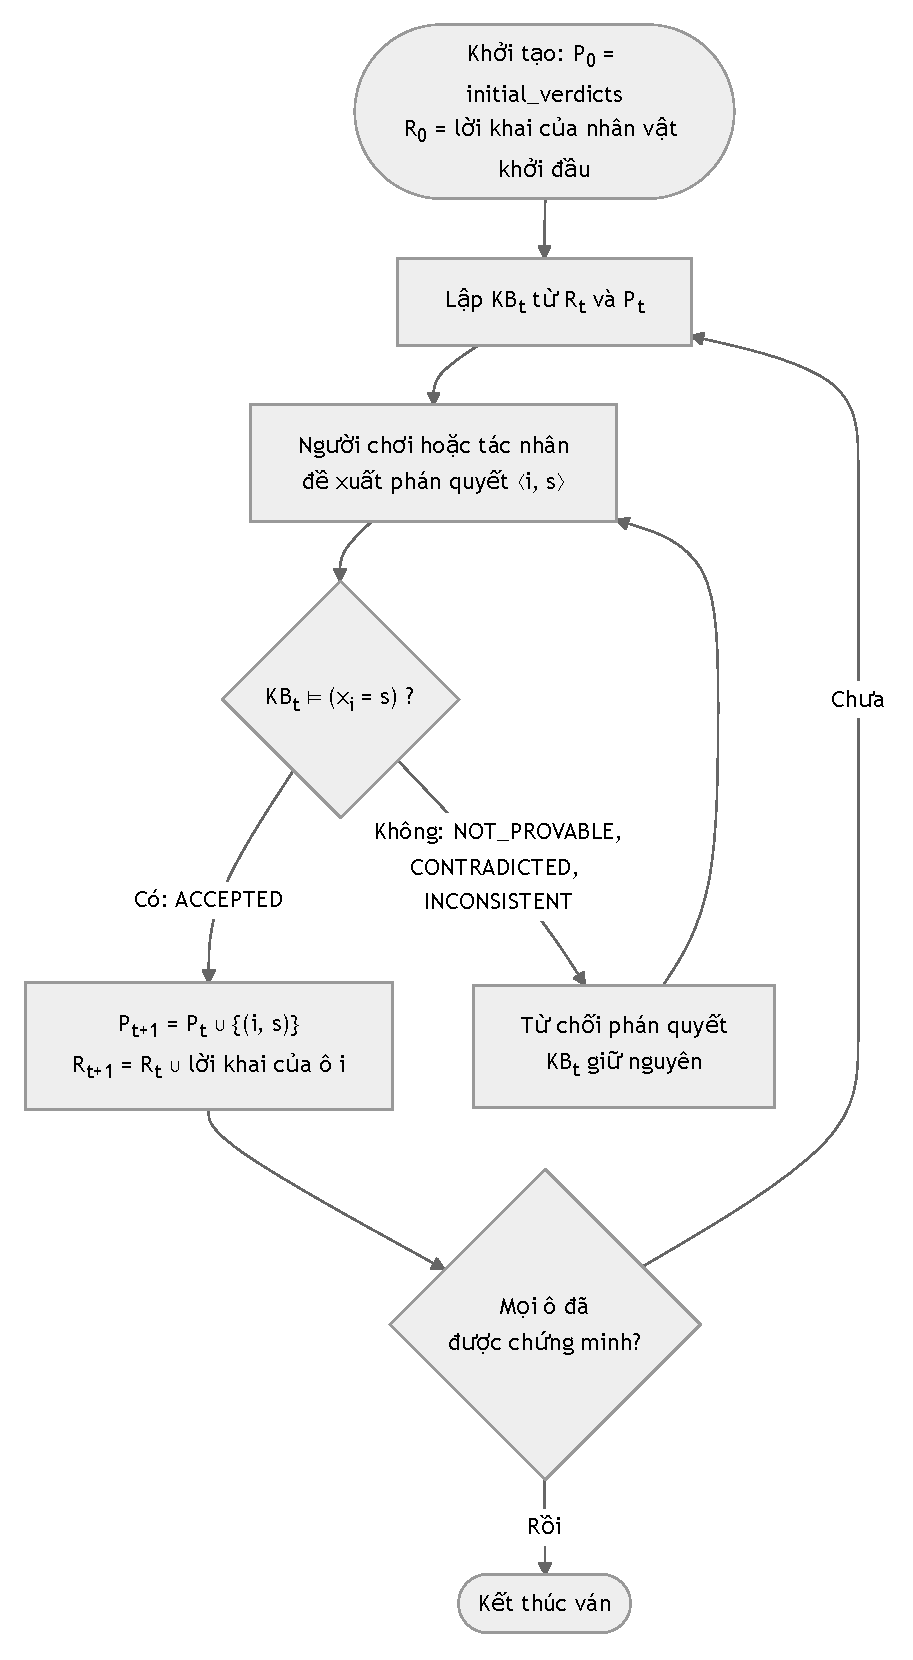
\includegraphics[width=0.62\linewidth]{figures/reveal_loop.pdf}
  \caption{Vòng lặp phán quyết và lật mở lời khai. Chỉ phán quyết được
    $\mathit{KB}_t$ suy ra tất yếu mới làm thay đổi trạng thái; mọi phán quyết
    khác bị từ chối và $\mathit{KB}_t$ giữ nguyên.}
  \label{fig:reveal_loop}
\end{figure}
